\documentclass[a4paper]{article}

\usepackage{amsfonts}
\usepackage{amsmath}
\usepackage{amsthm}
\usepackage[title]{appendix}
\usepackage[affil-it]{authblk}
\usepackage[margin=1in]{geometry}
\usepackage{graphicx}
\usepackage{hyperref}
\usepackage{mathrsfs}
\usepackage{multirow}
\usepackage{tikz}

\usepackage{clrscode}

\usetikzlibrary{shapes}

\setlength{\parskip}{3pt}

\DeclareGraphicsExtensions{.pdf}

\newtheorem{theorem}{Theorem}[section]

\begin{document}
    \title{One-Way Quantum Communication Complexity}
    \author{Dominic Moylett\thanks{\texttt{\href{dominic.moylett@bristol.ac.uk}{dominic.moylett@bristol.ac.uk}}}}
    \affil{Quantum Engineering Centre for Doctoral Training,\\University of Bristol}
    \date{\today}
    \maketitle

    \section{Introduction}

        Ever since the idea of quantum computing was first suggested, one of the most important questions has been ``What advantages would a quantum computer have over classical computers?'' In the decades that followed, quantum computers have shown many benefits, from factoring integers \cite{Shor:1997:PAP:264393.264406} to searching data \cite{Grover:1996:FQM:237814.237866} and even secure communication \cite{Bennett20147}. Given that quantum computers have shown such advantages for a single computer setting, a natural question is can they show advantages in distributed computation?

        We can evaluate the advantage of distributed quantum computation via communication complexity. Communication complexity is a very powerful model -- enough to earn its creator the first Knuth Prize\footnote{\url{http://www.sigact.org/Prizes/Knuth/1996.html}.} -- and has proven lower bounds in a wide variety of models. It has also led to applications in different forms of computation, from secure multi-party computation to data streaming. But finding separations is not easy, and Holevo's theorem has from the beginning shown us that there are problems which cannot be solved more efficiently via quantum communication.

        We will explore communication complexity in this report, focusing specifically on quantum advantages in the one-way communication setting. Section~\ref{sec:cc} offers a brief overview of communication complexity, and an explanation of Holevo's theorem. Section~\ref{sec:separations} provides examples of problems for which a separation between quantum and classical communication is either proven or conjectured. We conclude in Section~\ref{sec:conclusion} with a summary of the results and some open questions.

    \section{Communication Complexity}
    \label{sec:cc}

        Communication complexity was developed by Yao in 1979 as an analysis of distributed computing \cite{Yao:1979:CQR:800135.804414}. Under this model, our computation is done between two parties, commonly referred to as Alice and Bob, with inputs $x, y \in \{0, 1\}^n$, respectively. The two parties do not know each other's inputs; Alice does not know $y$ and Bob does not know $x$. Alice and Bob then exchange a series of messages between each other through a known protocol, with their aim being to jointly compute $f(x, y)$. The question communication complexity asks is how many bits of information do Alice and Bob need to communicate in order for them. We offer a sketch of a typical communication complexity problem in Figure~\ref{fig:cc}.

        A na\"{i}ve solution to any communication complexity problem uses $n$ bits of communication: Alice sends $x$ to Bob and Bob computes $f(x, y)$, possibly sending the result back to Alice. So the question is ``Can we compute $f(x, y)$ with $o(n)$ bits of communication?''

        One of the key benefits to communication complexity is that it is a useful model for proving lower bounds, and there are a number of established techniques for doing so. Lower bounds in communication complexity have also led to bounds in the data streaming model of computation\footnote{See \cite{TCS-002} for an explanation of the data streaming model.} such as in \cite{Gavinsky:2007:ESO:1250790.1250866} \& \cite{Verbin:2011:SCC:2133036.2133038}, as well as lower bounds for quantum and classical circuit depth \cite{MSC:4265920, 366852}. Beyond the computation of lower bounds, other applications to communication complexity include classical security \cite{Gavinsky:2007:ESO:1250790.1250866} and secure multiparty computation in both classical and quantum settings \cite{Franklin:1992:CCS:129712.129780, Data2014, 1409.8488}.

        \begin{figure}
            \centering
            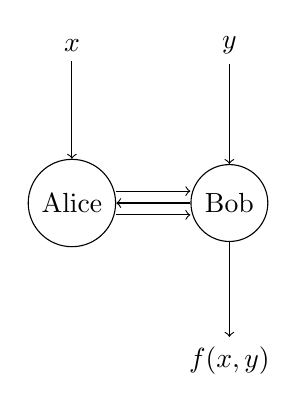
\begin{tikzpicture}[->, draw, node distance=2cm]
                \node[circle, draw] (Alice) at (0,0) {Alice};
                \node[circle, draw] (Bob) [right of=Alice] {Bob};
                \node (x) [above of=Alice] {$x$};
                \node (y) [above of=Bob] {$y$};
                \node (bout) [below of=Bob] {$f(x, y)$};
                \path
                    (x) edge (Alice)
                    (y) edge (Bob)
                    (Bob) edge (bout);
                \path ([yshift=1ex]Alice.east) edge ([yshift=1ex]Bob.west);
                \path (Bob.west) edge (Alice.east);
                \path ([yshift=-1ex]Alice.east) edge ([yshift=-1ex]Bob.west);
            \end{tikzpicture}
            \caption{An example of communication complexity. Alice and Bob begin computation with bit strings $x$ and $y$. They then exchange a series of messages based on a pre-determined protocol. Computation completes when Bob outputs $f(x, y)$.}
            \label{fig:cc}
        \end{figure}

        In one-way communication complexity, Alice and Bob again receive respective inputs $x, y \in \{0, 1\}^n$ with the aim being for Bob to output $f(x, y)$ for some function $f$. The difference now is that only one message is allowed to be sent from Alice to Bob, and Bob cannot send any messages to Alice.

        \subsection{Quantum Communication Complexity}

        In quantum communication complexity, first proposed in 1993 by Yao \cite{366852}, we also have parties Alice and Bob given inputs $x$ and $y$, respectively, who have to compute $f(x, y)$ for some function $f$. But now our two parties can send quantum messages between each other, and the complexity is measured in the number of qubits that are communicated.

        Another model by Cleve and Buhrman \cite{PhysRevA.56.1201} does not use the physical sending of data between the parties, but instead uses the measurement of entangled particles for remote computation. While our focus for this report however will be on the former, it is possible to simulate communicating $l$ individual qubits by use of $l$ entangled pairs and $2l$ classical bits of communication, via quantum teleportation \cite{PhysRevLett.70.1895}. Likewise, it is possible to simulate this model by the ability to communicate quantum states: Alice generates entangled pairs of qubits and sends one of the pair to Bob. This and other models are briefly discussed in Appendix~\ref{sec:other-models}.

        Because of the well-established techniques for lower-bounding classical communication complexity, a common area of research is to see if there are any problems which quantum protocols can solve by communicating fewer qubits than the number of classical bits required by lower bounds. Finding quantum protocols that beat classical lower bounds can give us intuition on the difference between quantum and classical encoding of data. These protocols will be the focus of Section~\ref{sec:separations}.

        \subsection{Holevo's Theorem}

        Even before Yao's work on the formalisation of Communication Complexity, it was clear that quantum communication would not be able to speed up some problems. A result by Holevo \cite{Hol73} gave an upper limit on the amount of information that can be extracted from a quantum state. A consequence of Holevo's theorem was that while a message of $n$ bits could be compressed into a message of less than $n$ qubits, the same message could not be retrieved from said qubits with absolute certainty. We phrase this as a communication complexity problem below.

        \begin{codebox}
            \Procname{Problem $\proc{COMMUNICATION}$}
            \zi \const{Alice's input:} $x \in \{0, 1\}^n$.
            \zi \const{Bob's input:} none.
            \zi \const{Bob's output:} $x$.
        \end{codebox}

        \begin{theorem}
            \label{thm:nayak}
            Any quantum protocol for COMMUNICATION that uses $O(m)$ qubits of communication succeeds with probability at most $2^{m-n}$.
        \end{theorem}

        We can prove Theorem~\ref{thm:nayak} by Holevo's theorem, but a later proof by Nayak \cite{814608} explains this result explicitly for encoding classical data in quantum data. This proof is given in Appendix~\ref{sec:nayak}.

        The only exception to this is if Alice and Bob have shared entangled qubits between each other prior to computation, in which case superdense coding can be used to communicate two bits by physically sending one qubit \cite{PhysRevLett.69.2881}. On the other hand, if Alice and Bob share prior entanglement and can communicate classically, they can communicate single qubits by physically sending pairs of bits \cite{PhysRevLett.70.1895}, so we can only save at most a factor of $1/2$ \cite{quant-ph/0101005}.

        Holevo's Theorem has in turn led to communication complexity problems which cannot be solved more efficiently with quantum communication. One example of this is the Inner Product problem:

        \begin{codebox}
            \Procname{Problem $\proc{INNER-PRODUCT}$}
            \zi \const{Alice's input:} $x \in \{0, 1\}^n$.
            \zi \const{Bob's input:} $y \in \{0, 1\}^n$.
            \zi \const{Bob's output:} $\sum_{i = 0}^{n - 1}x_i.y_i (\textrm{mod} 2)$.
        \end{codebox}

        Cleve et al.~\cite{Cleve201311} showed that if we were able to solve this problem in less than $O(n)$ qubits of communication, then it would be possible for Alice to communicate $x$ to Bob in $o(n)$ qubits, thus violating Holevo's theorem.

    \section{Separations Between Quantum and Classical Communication Complexity}
    \label{sec:separations}

        While it is clear from Holevo's theorem that we cannot solve all problems in fewer qubits than we can in classical bits, there are a number of problems which can be solved by communicating fewer qubits than classical bits. Some of the significant results are described in this section.

        \subsection{Distributed Deutsch-Jozsa}

        The Distributed Deutsch-Jozsa problem, first introduced by Buhrman, Cleve and Wigderson \cite{Buhrman:1998:QVC:276698.276713}, was the first example of an exponential separation between quantum and classical computation complexity. Prior to this, the largest gaps between classical and quantum communication were constant factors \cite{PhysRevA.56.1201}. The problem, and its quantum protocol as described in Buhrman et al.~\cite{RevModPhys.82.665}, are stated as follows, where $d(x, y)$ is the Hamming distance between $x$ and $y$ and $U_x = \sum_{i=0}^{n-1}(-1)^{x_i}|i\rangle\langle i|$ for $x \in \{0, 1\}^n$:

        \begin{codebox}
            \Procname{Protocol $\proc{DISTRIBUTED DEUTSCH-JOZSA}$}
            \zi \const{Alice's input:} $x \in \{0, 1\}^n$.
            \zi \const{Bob's input:} $y \in \{0, 1\}^n$.
            \zi \const{Promise:} $x = y$ or $d(x, y) = n/2$.
            \zi \const{Bob's output:} $0$ iff $x = y$, $1$ otherwise.
            \li Alice starts computation in the $|0\rangle^{\otimes \log n}$ state and applies $U_xH^{\otimes \log n}$ to get the state $|\psi\rangle$.
            \li Alice sends $|\psi\rangle$ to Bob.
            \li Bob applies $H^{\otimes \log n}U_y$ and measures in the computational basis.
            \li Bob outputs $0$ if they measure $|0\rangle^{\otimes \log n}$ and 1 otherwise.
            \End
        \end{codebox}

        The state Alice sends to Bob is $|\psi\rangle = \frac{1}{\sqrt{n}}\sum_{i=0}^{n-1} (-1)^{x_i}|i\rangle$. When Bob applies $U_y$ to this state, they end up with the state $\frac{1}{\sqrt{n}}\sum_{i=0}^{n-1}(-1)^{x_i}(-1)^{y_i}|i\rangle$. We'll now consider this state for two situations: one where $x = y$ and one where they differ in $n/2$ places, denoted $|\psi_0\rangle$ and $|\psi_1\rangle$, respectively.

        Note that if $x = y$ then $(-1)^{x_i}(-1)^{y_i} = 1$, so $|\psi_0\rangle = \frac{1}{\sqrt{n}}\sum_{i = 0}^{n-1}|i\rangle$. $|\psi_1\rangle$ on the other hand will have exactly $n/2$ amplitudes which are positive, and $n/2$ amplitudes which are negative. From this we can see that $\langle\psi_0|\psi_1\rangle = \frac{n/2 - n/2}{n} = 0$, so the states can be distinguished from one another upon measurement. Finally, Bob's application of $H^{\otimes \log n}$ converts their state to the computational basis. Note that $H|\psi_o\rangle = |0\rangle^{\otimes\log n}$, so measuring this state will indicate that $x = y$ and any other state will indicate that $d(x, y) = n/2$.

        So we have been able to deterministically solve this problem with $O(\log n)$ qubits of communication between Alice and Bob. How much classical communication is required to solve it? Buhrman et al.\cite{RevModPhys.82.665} used the work of Buhrman, Cleve and Wigderson \cite{Buhrman:1998:QVC:276698.276713} to give the following lower bound:

        \begin{theorem}
            \label{thm:ddj}
            The Distributed Deutsch-Jozsa Function requires $\Omega(n)$ bits of classical communication to be solved deterministically.
        \end{theorem}

        A summary of this proof is in Appendix~\ref{sec:ddj-lower-bound}. Thus we have an exponential gap between deterministic classical communication and quantum communication for the Distributed Deutsch-Jozsa problem. However, this quantum advantage is lost when compared to randomised classical communication: Alice picks a random index $i \in \{0,...,n-1\}$ and sends $(i, x_i)$ to Bob, who outputs $0$ if $x_i = y_i$ and $1$ otherwise. This protocol has error $1/2$, which can be reduced by repetition. Overall communication is $O(\log n)$ bits.

        \subsection{Subgroup Membership}
        \label{sec:subgroup-membership}

        Another disadvantage with the Distributed Deutsch-Jozsa problem is that it is a partial function, in that it requires a promise. This begs the question: Are there any functions which do not rely on promises -- better known as total functions -- but still have a quantum advantage?

        This is an open question, but some progress has been made. Aaronson et al.~\cite{0902.3175} explored the problem of subgroup membership as potentially yielding a quantum advantage for a total function. Their protocol for solving subgroup membership, based on an earlier algorithm by Watrous \cite{Watrous:2000:SQP:795666.796590}, is described below, where $G$ is a group, $\mathscr{H}_G$ is the set of all subgroups of $G$, $|+\rangle = \frac{1}{\sqrt{2}}(|0\rangle + |1\rangle)$ and $U_{G, y} = \sum_{g \in G}|yg\rangle\langle g|$ for some $y \in G$:

        \begin{codebox}
            \Procname{Protocol $\proc{SUBGROUP-MEMBERSHIP}$}
            \zi \const{Alice's input}: $H \in \mathscr{H}_G$.
            \zi \const{Bob's input}: $y \in G$.
            \zi \const{Bob's output}: $1$ if $y \in H$, $0$ otherwise.
            \li Alice prepares the state $|H\rangle = \frac{1}{\sqrt{|H|}}\sum_{h \in H}|h\rangle$, which is then sent to Bob.
            \li Bob prepends an ancilla qubit to get $|H\rangle|+\rangle$ and applies $U_{G, y}$ controlled on the final qubit.
            \li Bob applies a Hadamard to the second qubit and measures in the computational basis.
        \end{codebox}

        Any element $h \in H$ can be described in $\lceil\log |G|\rceil$ bits, so Alice needs to send $O(\log |G|)$ qubits to Bob in order to perform this protocol.

        After line 2, Bob has the state $\frac{1}{\sqrt{2}}(|H\rangle|0\rangle + |yH\rangle|1\rangle)$, where $|yH\rangle = \frac{1}{\sqrt{|H|}}\sum_{h \in H}|yh\rangle$. If $y \in H$ then $U_{G, y}|H\rangle|+\rangle = |H\rangle|+\rangle$, so applying a Hadamard to the final qubit makes the final qubit $|0\rangle$. A measurement in the computational basis will thus always yield $0$.

        On the other hand, if $y \notin H$ then $\langle yH|H\rangle = 0$, so applying the Hadamard produces

        $$\frac{1}{2}((|H\rangle + |yH\rangle)|0\rangle + (|H\rangle - |yH\rangle)|1\rangle).$$

        Measuring the ancilla qubit will result in $|0\rangle$ -- and thus a false positive -- with probability $1/2$. We can repeat this protocol a constant number of times to reduce this error.

        Classically, it has been shown by Miltersen et al.~\cite{Miltersen199837} that any one-way randomised protocol with completeness probability of $1/2$ and perfect soundness must use $\Omega(\log^2|G|)$ bits of communication. Aaronson et al.~ have conjectured that this bound still holds even in a bounded-error setting.

        So if we can find a total subgroup membership function that cannot classically be solved using $O(\log |G|)$ bits of communication, then we will have a polynomial gap for a total function. The problem is that there are many subgroups which can be solved classically. For example, Aaronson et al.~gave the following theorem for normal subgroups:

        \begin{theorem}
            \label{thm:norm-sg-membership}
            For normal subgroup $H \in \mathscr{H}_G, y \in G$ there is an $O(\log|G|)$ protocol which outputs with probability $1$ if $y \in H$ and $0$ with probability at least $1/2$ if $y \notin H$.
        \end{theorem}

        To explain this classical protocol, we first need to describe complex characters. For any complex field representation $\rho$ of $G$, the complex character $\chi$ is the function $\chi(g) = \textrm{tr}(\rho(g))~\forall~g\in G$. For any two elements $g, g' \in G$, we have the relation that $\chi(gg'g^{-1}) = \chi(g)$. If $1$ is the identity elemnent of $G$, then $\chi(1)$ is the dimension of $\rho$, and the kernel of $\chi$, denoted $\textrm{ker}(\chi) = \{g \in G|\chi(g) = \chi(1)\}$. If $\rho$ is irreducible then $\chi$ is an irreducible character, and the set of irreducible complex characters of $G$ is denoted $\textrm{Char}(g)$. If $H$ is a normal subgroup of $G$, then let

        $$\Lambda_H = \{\chi \in \textrm{G}|H\subseteq \textrm{ker}(\chi)\}.$$

        Given this definition we note that

        $$\sum_{\chi \in \Lambda_H}[\chi(1)]^2 = \frac{|G|}{|H|}.$$

        We now describe the protocol from Aaronson et al.~\cite{0902.3175}:

        \begin{codebox}
            \Procname{Protocol $\proc{NORMAL-SUBGROUP-MEMBERSHIP}$}
            \zi \const{Alice's input}: $H \in \mathscr{H}_G$ such that $H$ is normal.
            \zi \const{Bob's input}: $y \in G$.
            \zi \const{Bob's output}: $1$ if $y \in H$, $0$ otherwise.
            \li Alice chooses a random complex character $\mu$ such that $H \subseteq \textrm{ker}(\mu)$ with probability $\frac{|H|}{|G|}[\mu(1)]^2$.
            \li Alice sends $\mu$ to Bob.
            \li Bob outputs $1$ if $y \in \textrm{ker}(\mu)$ and $0$ otherwise.
        \end{codebox}

        \begin{proof}[Proof of Theorem~\ref{thm:norm-sg-membership}]
        If $y \in H \subseteq \textrm{ker}(\mu)$ then $\mu(y) = \mu(1)$ and thus the protocol will succeed. So the protocol fails if Alice picks a character $\mu$ such that $y \in \textrm{ker}(\mu) \setminus H$. We shall call the set of all characters that would cause an error $B$. Based on Alice's selection probability, the probability of an error is thus

        $$\frac{|H|}{|G|}\sum_{\chi \in B}[\chi(1)]^2.$$

        To analyse this further, we will look at the smallest normal subgroup of $G$ which contains both $H$ and $y$. We will call this subgroup $K$, which can be stated formally as $K = \{gkg^{-1}|g \in G, k \in H \cup \{y\}\}$. Note that $|K| \geq 2|H|$, as $h \in K$ and $hyh^{-1} \in K$, but $hyh^{-1} \notin H ~\forall~h\in H$.

        The final point we will need is that $B \subseteq \Lambda_K$. Consider a character $\chi \in B$. Because $\chi$ could be selected by Alice, we know that $H \subseteq \textrm{ker}(\chi)$. We also know that $y \in \textrm{ker}(\chi)$ because $\chi \in B$. We see from this that any other element in $K$ must also be in $\textrm{ker}(\chi)$, as $\chi(gkg^{-1}) = \chi(k)~\forall~g\in G, k\in H \cup \{y\}$. Thus $K \subseteq \textrm{ker}(\chi)$ and we can conclude that $\chi \in \Lambda_K$.

        Using the above points, we can show that

        $$\frac{|H|}{|G|}\sum_{\chi \in B}[\chi(1)]^2 \leq \frac{|H|}{|G|}\sum_{\chi \in \Lambda_K}[\chi(1)]^2 = \frac{|H|}{|G|}\frac{|G|}{|K|} \leq \frac{|H|}{2|H|} = \frac{1}{2}.$$

        Thus this protocol fails with probability at most $1/2$. Finally, we note that is is possible to describe $\mu$ in $\lceil\log|G|\rceil$ bits, as $\mu \in \Lambda_H$ and $|\lambda_H| \leq |Char(G)| \leq |G|$.
        \end{proof}

        Other groups also proven to be solvable in $(O\log|G|)$ bits of communication include groups with small modular or representations and groups with small complex representations \cite{0902.3175}. So already we have three cases of groups which don't have a separation.

        \subsection{Hidden Matching}
        \label{sec:hidden-matching}

        A matching $M$ is a sequence of $k$ disjoint pairs $(i_1, j_1), (i_2, j_2),...,(i_k, j_k) \in [n]^2$. A matching is said to be partial if some indexes do not appear in any pair, and perfect if each integer appears in exactly one pair. A matching $M$ together with an $n$-bit string $x$ define a $k$-bit string as follows:

        $$Mx = (x_{i_1} \oplus x_{j_1}), (x_{i_2} \oplus x_{j_2}), ... (x_{i_k} \oplus x_{j_k})$$

        The Hidden Matching problem was first investigated in terms of one-way communication complexity in \cite{doi:10.1137/060651835}. The problem and its quantum protocol are defined below, where $\mathcal{M}_n$ is the set of perfect matchings on $n$-node graphs:

        \begin{codebox}
            \Procname{Protocol $\proc{HIDDEN-MATCHING}$}
            \zi \const{Alice's input}: $x \in \{0,1\}^n$.
            \zi \const{Bob's input}: $M \in \mathcal{M}_n$.
            \zi \const{Bob's output}: $(i, j, x_i\oplus x_j)$ for some $(i, j) \in M$.
            \li Alice prepares the state $|x\rangle = \frac{1}{\sqrt{n}}\sum_{i = 0}^{n - 1}(-1)^{x_i}|i\rangle$, which is then sent to Bob.
            \li Bob measures $|x\rangle$ in the $\{\frac{1}{\sqrt{2}}(|i\rangle\pm|j\rangle)|(i, j) \in M\}$ basis and gets the state $|\psi_{i\pm j}\rangle$.
            \li Bob returns $(i, j, b)$, where $b = 0$ if $|\psi_{i\pm j}\rangle = \frac{\pm 1}{\sqrt{2}}(|i\rangle+|j\rangle)$ and $b = 1$ if $|\psi_{i\pm j}\rangle = \frac{\pm 1}{\sqrt{2}}(|i\rangle-|j\rangle)$.
        \end{codebox}

        First, note that since $M$ is a perfect matching, each index $i \in \{0,...,n-1\}$ occurs in exactly one $(i, j)$-pair in $M$. Thus the basis of step $2$ is orthonormal and can be measured. The probability of measuring $|\psi_{i \pm j}\rangle$ is

        $$P(i\pm j) = \left|\frac{1}{\sqrt{n}}\sum_{k=0}^{n-1}(-1)^{x_k}\frac{1}{\sqrt{2}}(|i\rangle \pm |j\rangle)\right|^2 = \frac{|(-1)^{x_i} \pm (-1)^{x_j}|^2}{2n}$$.

        If $x_i \oplus x_j = 0$ then $x_i = x_j$, so $P(i-j) = \frac{1}{2n}(1-1) = 0$ and thus Bob will measure the state $|\psi_{i+j}\rangle$. Likewise, if $x_i \oplus x_j = 1$ then Bob will measure the state $|\psi_{i-j}\rangle$. Thus this quantum protocol will always find a pair, though a specific pair has probability $\frac{1}{2n}$.

        As for classical one-way protocols, the following theorem was proven in \cite{doi:10.1137/060651835}:

        \begin{theorem}
            \label{thm:hm}
            A random one-way protocol for the Hidden Matching problem with deterministic Alice requires $O(\sqrt{n})$ bits of communication.
        \end{theorem}

         This proof is summarised in Appendix~\ref{sec:hm-lower-bound}.

        Unfortunately, this is not an example of a total function that separates quantum and classical one-way communication complexity. This is because the hidden matching problem has a one-to-many mapping: Bob is allowed to output any $(i, j, x_i \oplus x_j)$ tuple under the condition that $(i, j) \in M$, thus there are $n/2$ acceptable outputs. This makes the hidden matching problem not a function, but a relation. A separation for relations does not necessarily prove a separation for functions.

        \subsection{$\alpha$-Matching}

        $\alpha$-Matching is a promise function related to the hidden matching problem. In $\alpha$-matching, the matching given to Bob consists of $\alpha n$ disjoint pairs. If $\alpha = 1/2$ then the matching is perfect like before, and if $\alpha < 1/2$ then the matching is partial. The problem and its quantum protocol from \cite{Gavinsky:2007:ESO:1250790.1250866} are described as follows, where $\mathcal{M}_{\alpha n}$ is the set of all $\alpha$-matchings, and $\bar{x}$ is the bitwise NOT of the string $x$:

        \begin{codebox}
            \Procname{Protocol $\proc{$\alpha$-MATCHING}$}
            \zi \const{Alice's input}: $x \in \{0,1\}^n$.
            \zi \const{Bob's input}: $M \in \mathcal{M}_{\alpha n}, w \in \{0, 1\}^{\alpha n}$.
            \zi \const{Promise}: $w = Mx$ or $\bar{w} = Mx$.
            \zi \const{Bob's output}: $0$ if $w = Mx$, $1$ otherwise.
            \li Bob adds $(i, j)$ pairs to their matching to get perfect matching $M'$.
            \li Alice and Bob run the HIDDEN-MATCHING protocol on $(x, M')$ to get tuple $(i, j, b)$.
            \li If $(i, j) \notin M$ then Bob aborts.
            \li Bob outputs $0$ if $w_k = b$ and $1$ otherwise.
        \end{codebox}

        First note that Bob only needs one bit of $Mx$ to figure out which of the two cases holds because of the promise. So if we can find one pair $(x_i, x_j)$ such that $(i, j) \in M$, then we have solved this problem. Since the pairs in $M$ are disjoint, we can pad $M$ with extra pairs to get a reduction to the Hidden Matching problem.

        The only case where we will fail is if the hidden matching protocol returns $(i, j, x_i \oplus x_j)$ such that $(i, j) \notin M$. We can reduce this probability by repeating the protocol $O(k/\alpha)$ times for some $k \ll \alpha n$ to get a high probability of successfully finding one bit of $Mx$ with $O(\log n)$ bits of communication.

        So how well can we solve this problem with classical communication? Gavinsky et al.~\cite{Gavinsky:2007:ESO:1250790.1250866} proved the following:

        \begin{theorem}
            A random one-way protocol for $\alpha$-Matching problem with deterministic Alice requires $\Omega(\sqrt{n/\alpha})$ bits of communication.
        \end{theorem}

        \begin{proof}
        We can prove this by asking how much Bob can learn if Alice sends him $c$ bits, where $1 \leq c \leq \gamma \epsilon\sqrt{n/\alpha}$, for some $\epsilon > 0, \alpha \in (0,1/4]$ and a carefully chosen value of $\gamma$ which will be used later.

        If Alice's message is deterministic based on $x$, then the $c$ bits Alice sends allows Bob to define a set $A \subseteq \{0, 1\}^n$ such that $|A| \geq 2^{n-c}$ of bit strings from which Bob must be able to guess Alice's input $x$. The probability of Bob succeeding then is the probability of him picking a bit string $x' \in A$ such that $Mx = Mx'$. We define the probability of Bob finding a string $x$ such that $Mx = z$ for some $k$-bit string $z$ as

        $$p_M(z) = \frac{|\{x \in A|Mx = z\}|}{|A|}.$$

        Gavinsky et al.~showed that as Alice's message becomes shorter than $O(\sqrt{n/\alpha})$, this probability distribution becomes arbitrarily close to the uniform distribution. They start by looking at the expected value of the squared total variational distance between the probability distribution and the uniform distribution:

        $$\mathbb{E}_M[\|p_M - U\|_{tvd}^2] = \mathbb{E}_M[(\sum_{z \in \{0, 1\}^{\alpha n}}|p_M(z) - U(z)|)^2]$$

        This can then be re-written as a squared inner product:

        $$2^{2\alpha n}\mathbb{E}_M\left[\left(\frac{1}{2^{\alpha n}}\sum_{z \in \{0, 1\}^{\alpha n}}1 * |p_M(z) - U(z)|\right)^2\right] = 2^{2\alpha n}\mathbb{E}_M[\langle 1, |p_M(z) - U(z)|\rangle^2]$$

        where $1$ is the function $1(z) = 1~\forall~z\in\{0, 1\}^{\alpha n}$ and $\langle f, g\rangle = \frac{1}{2^{\alpha n}}\sum_{z \in \{0, 1\}^{\alpha n}}f(z)g(z)$ is the inner product. By the Cauchy-Schwarz inequality, we can bound this value:

        $$2^{2\alpha n}\mathbb{E}_M[\langle 1, |p_M(z) - U(z)|\rangle^2] \leq 2^{2\alpha n}\mathbb{E_M}[\|1\|_2^2\|p_M - U\|_2^2] = 2^{2\alpha n}\mathbb{E}_M[\|p_M - U\|_2^2]$$

        where $\|f\|_2^2 = \langle f, f\rangle$ is the $l_2$-norm. We then use Parseval's identity and note that $\widehat{U}(z) = \widehat{f}(z) = 2^{-\alpha n}$ if $z = 0$ and $\widehat{U}(z) = 0$ otherwise.

        $$2^{2\alpha n}\mathbb{E_M}[\|p_M - U\|_2^2] = 2^{2\alpha n}\mathbb{E}_M\left[\sum_{z \in \{0, 1\}^{\alpha n}}(\widehat{p_M}(z) - \widehat{U}(z))^2\right] = 2^{2\alpha n}\mathbb{E}_M\left[\sum_{z \in \{0, 1\}^{\alpha n}\setminus\{0^{\alpha n}\}}\widehat{p_M}(z)^2\right]$$

        where $\widehat{f}(z) = \sum_{y \in \{0, 1\}^{\alpha n}}f(y)(-1)^{x.y}$ is the Fourier transform of $f$ and $.$ is the dot product. Now let us look at the fourier transform of $p_M$:

        \begin{align*}
            \widehat{p_M}(z) &= \frac{1}{2^{\alpha n}}\sum_{s \in \{0, 1\}^{\alpha n}}p_M(s)(-1)^{s.z}\\
            &= \frac{1}{|A|2^{\alpha n}}\sum_{s \in \{0, 1\}^{\alpha n}}|\{y \in A|My = s\}|(-1)^{s.z}\\
            &= \frac{1}{|A|2^{\alpha n}}\sum_{s \in \{0, 1\}^{\alpha n}}|\{y \in A|My = s\}|(-1)^{My.z}
        \end{align*}

        Note that for any given $y \in A$, there is exactly one $s \in \{0, 1\}^{\alpha n}$ such that $My = s$. Because we are summing over all $\alpha n$-bit strings, we are essentially summing over all $y \in A$:

        \begin{align*}
            \widehat{p_M}(z) &= \frac{1}{|A|2^{\alpha n}}\sum_{s \in \{0, 1\}^{\alpha n}}|\{y \in A|My = s\}|(-1)^{My.z}\\
            &= \frac{1}{|A|2^{\alpha n}}\sum_{y \in A}(-1)^{My.z}\\
            &= \frac{1}{|A|2^{\alpha n}}\sum_{y \in A}(-1)^{y.M^Tz}\\
            &= \frac{1}{|A|2^{\alpha n}}\sum_{y \in \{0, 1\}^n}1_A(y)(-1)^{y.M^Tz}\\
            &= \frac{2^n}{|A|2^{\alpha n}}\widehat{1_A}(M^Tz)
        \end{align*}

        where $1_A$ is the indicator function of $A$. Plugging this back into our formula, we find that

        $$2^{2\alpha n}\mathbb{E}_M\left[\sum_{z \in \{0, 1\}^{\alpha n}\setminus\{0^{\alpha n}\}}\widehat{p_M}(z)^2\right] = \frac{2^{2n}}{|A|^2}\mathbb{E}_M\left[\sum_{z \in \{0, 1\}^{\alpha n}\setminus\{0^n\}}\widehat{1_A}(M^Tz)^2\right].$$

        Next, we move from summing over $\alpha n$-bit strings to summing over $n$-bit strings, and note that the set $V = |\{s \in \{0, 1\}^{\alpha n}|M^Ts = v\}| \leq 1 ~\forall~ v \in \{0, 1\}^n$. This means that our expectation over $M$ is a probability:

        \begin{align*}
            \frac{2^{2n}}{|A|^2}\mathbb{E}_M\left[\sum_{z \in \{0, 1\}^{\alpha n}\setminus\{0^n\}}\widehat{1_A}(M^Tz)^2\right] &= \frac{2^{2n}}{|A|^2}\mathbb{E}_M\left[\sum_{v \in \{0, 1\}^n\setminus\{0^n\}}|\{s \in \{0, 1\}^{\alpha n}|M^Ts = v\}|\widehat{1_A}(v)^2\right]\\
            &= \frac{2^{2n}}{|A|^2}\sum_{v \in \{0, 1\}^n\setminus\{0^n\}}\mathrm{Pr}_M[\exists~ s \in \{0, 1\}^{\alpha n} \textrm{ s.t. } M^Ts = v]\widehat{1_A}(v)^2
        \end{align*}

        Now we need to consider what this probability over $M$ is. Suppose the Hamming weight of $v$ is $|v| = k$ for even $k$\footnote{The Hamming weight of $M^Ts$ is even and at most $2\alpha n$.}. Lemma 5 of \cite{Gavinsky:2007:ESO:1250790.1250866} showed that the fraction of $\alpha$-matchings which satisfy the probability is equal to the number of $\alpha n$-bit strings with Hamming weight $k/2$ over the number of $n$-bit strings with Hamming weight $k$:

        $$\frac{2^{2n}}{|A|^2}\sum_{v \in \{0, 1\}^n\setminus\{0^n\}}\mathrm{Pr}_M[\exists~ s \in \{0, 1\}^{\alpha n} \textrm{ s.t. } M^Ts = v]\widehat{1_A}(v)^2 = \frac{2^{2n}}{|A|^2}\sum_{\textrm{even }k=2}^{2\alpha n}\frac{\binom{\alpha n}{k/2}}{\binom{n}{k}}\sum_{v:|v| = k}\widehat{1_A}(v)^2$$

        At this point, we are going assume that $k \leq 4c$ and let $\delta = k/4c$. Because $\delta \in (0,1]$, we can apply the Kahn, Kalai and Linial inequality \cite{21923}:

        \begin{align*}
            \sum_{\textrm{even }k=2}^{4c - 2}\frac{\binom{\alpha n}{k/2}}{\binom{n}{k}}\frac{2^{2n}}{|A|^2}\sum_{v:|v| = k}\widehat{1_A}(v)^2 &\leq \sum_{\textrm{even }k=2}^{4c-2}\frac{\binom{\alpha n}{k/2}}{\binom{n}{k}}\frac{2^{2n}}{|A|^2}\frac{1}{\delta^k}\left(\frac{|A|}{2^n}\right)^{2/(1 + \delta)}\\
            &= \sum_{\textrm{even }k=2}^{4c - 2}\frac{\binom{\alpha n}{k/2}}{\binom{n}{k}}\frac{1}{\delta^k}\left(\frac{2^n}{|A|}\right)^{2\delta/(1 + \delta)}\\
        \end{align*}

        We bound this value by the following inequalities: $|A| \geq 2^{n - c}$, $(n/k)^k \leq \binom{n}{k} \leq (en/k)^k$ and $c \leq \gamma \epsilon \sqrt{n/\alpha}$:

        \begin{align*}
            \sum_{\textrm{even }k=2}^{4c - 2}\frac{\binom{\alpha n}{k/2}}{\binom{n}{k}}\frac{1}{\delta^k}\left(\frac{2^n}{|A|}\right)^{2\delta/(1 + \delta)} &\leq \sum_{\textrm{even }k=2}^{4c - 2}\frac{\binom{\alpha n}{k/2}}{\binom{n}{k}}\frac{1}{\delta^k}\left(\frac{2^n}{|A|}\right)^{k/2c}\\
            &\leq \sum_{\textrm{even }k=2}^{4c - 2}\frac{\binom{\alpha n}{k/2}}{\binom{n}{k}}\left(\frac{4\sqrt{2}c}{k}\right)^{k}\\
            &\leq \sum_{\textrm{even }k=2}^{4c - 2}\frac{(2e\alpha n)^{k/2}}{(n/k)^k}\left(\frac{4\sqrt{2}c}{k}\right)^{k}\\
            &\leq \sum_{\textrm{even }k=2}^{4c - 2}\left(\frac{64e\alpha c^2}{kn}\right)^{k/2} \leq \sum_{\textrm{even }k=2}^{4c - 2}\left(\frac{64e\gamma^2\epsilon^2}{k}\right)^{k/2}
        \end{align*}

        A small value for $\gamma$ will ensure that this sum is less than $\epsilon^2/2$.

        We now need to bound the sum for values of $k \geq 4c$. For this, we note that the term $\binom{\alpha n}{k/2}/\binom{n}{k}$ decreases as $k$ increases:

        \begin{align*}
            \frac{\binom{\alpha n}{k/2 - 1}/\binom{n}{k-2}}{\binom{\alpha n}{k/2}/\binom{n}{k}} &= \frac{(k/2)!(\alpha n - k/2)!}{(k/2 - 1)!(\alpha n - k/2 + 1)!}\frac{(k-2)!(n-k + 2)!}{k!(n-k)!}\\
            &= \frac{k/2}{\alpha n - k/2 + 1}\frac{(n - k + 1)(n - k + 2)}{k(k - 1)}\\
            &= \frac{(n - k + 2)(n - k + 1)}{(2\alpha n - k + 2)(k - 1)} \geq \frac{n - k + 1}{k - 1} \geq 1
        \end{align*}

        Plugging this in and recalling that $(n/k)^k \leq \binom{n}{k} \leq (en/k)^k$, we find that

        \begin{align*}
            \frac{2^{2n}}{|A|^2}\sum_{\textrm{even }k=4c}^{2\alpha n}\frac{\binom{\alpha n}{k/2}}{\binom{n}{k}}\sum_{v:|v| = k}\widehat{1_A}(v)^2 &\leq \frac{2^{2n}}{|A|^2}\sum_{\textrm{even }k=4c}^{2\alpha n}\frac{\binom{\alpha n}{2c}}{\binom{n}{4c}}\sum_{v:|v| = k}\widehat{1_A}(v)^2\\
            &= \frac{2^{2n}}{|A|^2}\left(\frac{8 e\alpha c}{n}\right)^{2c}\sum_{\textrm{even }k=4c}^{2\alpha n}\sum_{v:|v| = k}\widehat{1_A}(v)^2.
        \end{align*}

        Now we note by Parseval's identity that $\sum_{v \in \{0, 1\}^n}\widehat{1_A}(v)^2 = \|1_A\|_2^2 = |A|2^{-n}$, and recall that $|A| \geq 2^{n-c}$ and $c \leq \gamma \epsilon \sqrt{n/\alpha}$:

        $$\frac{2^{2n}}{|A|^2}\left(\frac{8 e\alpha c}{n}\right)^{2c}\sum_{\textrm{even }k=4c}^{2\alpha n}\sum_{v:|v| = k}\widehat{1_A}(v)^2 \leq \frac{2^n}{|A|}\left(\frac{8 e\alpha c}{n}\right)^{2c} \leq 2^c\left(\frac{8 e\alpha c}{n}\right)^{2c} \leq \left(\frac{8\sqrt{2} e\gamma\epsilon\sqrt{n}}{\sqrt{\alpha}}\right)^{2c}$$

        Again, this equation can be bounded by $\epsilon^2/2$ for small enough $\gamma$, as $\alpha/n < 1$, $c \geq 1$. By adding these two cases together, we find that the squared total variation distance is at most $\epsilon^2$. To conclude, we use Jensen's inequality:

        $$(\mathbb{E}_M[\|p_M - U\|_{tvd}])^2 \leq \mathbb{E}_M[\|p_M - U\|_{tvd}^2] \leq \epsilon^2$$

        We conclude that if Alice sends fewer than $\sqrt{n/\alpha}$ bits of classical data to Bob then this distribution is indistinguishable form uniform.
        \end{proof}

        One potential weakness with this proof is the use of $\gamma$, which is to essentially force the message to be small enough that this proof holds. It would be interesting to see to what extent we can bound this relation if $\gamma = 1$.

        A more general version of the problem was explored by Verbin and Yu in 2011 \cite{Verbin:2011:SCC:2133036.2133038}, where showed that $t$-dimensional hypermatching requires $\Omega(n^{1-1/t})$ bits of classical communication. Note that $t=2$ is consistent with Bar-Yossef, Jayram and Kerenidis' results for perfect matching \cite{doi:10.1137/060651835}.

        Another partial function related to both Subgroup Membership and $\alpha$-matching is Permutation Invariance \cite{Montanaro:2011:NES:2230916.2230919}, which is discussed in Appendix~\ref{sec:perm-invariance}.

    \section{Conclusion}
    \label{sec:conclusion}

        Communication complexity has proven itself to be a powerful tool in theoretical computer science, from its origins in distributed computation to lower bounds in the circuit depth \& streaming models alongside applications in cryptography. It has also proven over the last two and a half decades to be useful for finding separations between classical and quantum computing.

        We have presented in this report some of the one-way communication relations and partial functions for which the communication of bits is significantly worse than qubits. It is important to note that a number of other grand separations have also been proven which we have not been able to cover in this essay: Gavinsky \cite{gavinsky2008classical} showed a relation which had an exponential separation between one-way quantum communication and two-way randomised classical communication. Regev and Klartag \cite{Regev:2011:QOC:1993636.1993642} later showed a partial function with the same separation.

        While we have focused on one-way communication complexity as well as some of two-way in this conclusion, there are many other models of communication complexity with varying levels of power. Some of these are summarised in Appendix~\ref{sec:other-models}.

        \subsection{Open Problems}

        Alas, for all the successes we have seen in one-way communication complexity, finding a total function for which there exists an advantage for quantum communication is still open. Such an advantage would ideally be exponential, as a polynomial gap could be useless in practice if sending classical bits is cheaper \cite{RevModPhys.82.665}. But even finding a polynomial gap has proven to be a challenge.

        Aaronson and LeGall have made considerable headway towards finding a subgroup which cannot be solvable in $O(\log |G|)$ bits of communication, and conjecture that such a subgroup does exist \cite{0902.3175}. Indeed, Aaronson called the problem one of his Ten Semi-Grand Challenges\footnote{\url{http://www.scottaaronson.com/blog/?p=471}}.

        While the hidden subgroup problem might show a gap for one-way communication, there is an $O(\log|G|)$ protocol in two-way communication: Bob sends $g$ to Alice who sends back $0$ if $g \in H$ and $1$ otherwise. Thus we would still need a different problem in order to show even a separation for a total function between two-way randomised classical communication and one-way quantum communication.

    \bibliographystyle{alpha}
    \bibliography{quantum_communication_complexity}{}

    \begin{appendices}

    \section{Nayak's Proof of Quantum Communication Complexity}
    \label{sec:nayak}

    \begin{proof}[Proof of Theorem~\ref{thm:nayak}]
        Suppose we create an encoding $x \mapsto \{q_{x,i}|\phi_{x_i}\rangle\}$ such that $x$ is an $n$-bit string and $\{q_{x,i}|\phi_{x_i}\rangle\}$ is a mixed state over $m$ qubits. We decode this message by measuring over projection operators $\{P_x\}$. The mean probability of Bob successfully decoding an $x$ that has been selected uniformly at random is $2^{-n}\sum_{x, i}q_{x, i}\|P_x|\phi_{x,i}\rangle\|^2$. This can be bounded by making our states pure and setting $|\phi_x\rangle = \max_{|\psi_{x, i}\rangle}\|P_x|\phi_{x, i}\rangle\|^2$:

        $$\frac{1}{2^n}\sum_{x, i}q_{x, i}\|P_x|\phi_{x,i}\rangle\|^2 \leq \frac{1}{2^n}\sum_{x}\|P_x|\phi_{x}\rangle\|^2$$

        Next, we decompose $P_x$ into an orthonormal basis $\{|\hat{e}_{x, j}\rangle\}$ and create a subspace $E$ that spans the code words $\{|\phi_x\rangle\}$ with projection $Q$:

        $$\frac{1}{2^n}\sum_{x}\|P_x|\phi_{x}\rangle\|^2 = \frac{1}{2^n}\sum_{x, j}\langle\phi_x|\hat{e}_{x, j}\rangle\langle\hat{e}_{x, j}|\phi_x\rangle \leq \frac{1}{2^n}\sum_{x}\|Q|\hat{e}_{x, j}\rangle\|^2$$

        Finally, we decompose $Q = \sum_i|e_i\rangle\langle e_i|$ where $\{|e_i\rangle\}$ is an orthonormal basis spanning $E$. Note that since $|\phi_x\rangle$ is conveyed in at most $m$ qubits, $|\{|e_i\rangle\}| \leq 2^m$. Hence we conclude that

        $$\frac{1}{2^n}\sum_{x, j}\|Q|\hat{e}_{x, j}\rangle\|^2 \leq \frac{1}{2^n}\sum_{x, j, i}|\langle e_i|e_{x, j}\rangle|^2 \leq \frac{1}{2^n}\sum_{i}|\langle e_i|e_i\rangle|^2 \leq 2^{m - n}.$$
    \end{proof}

    \section{Distributed Deutsch-Jozsa Lower Bound}
    \label{sec:ddj-lower-bound}

    \begin{proof}[Proof of Theorem~\ref{thm:ddj}]
        To lower bound the Distributed Deutsch-Jozsa problem, denoted $DDJ$, we will partition the problem space up into rectangles $(a, b, c, d)$ such that $DDJ(x_i, y_i) = DDJ(x_i', y_i')$ for any pair of inputs $(x_i, y_i), (x_i', y_i') \in \{x_a,x_{a + 1},...,x_{b}\} \times \{y_c, y_{c+1},...,y_d\}$. We can lower bound the number of messages to $c$ bits if we need $2^c$ rectangles to cover the entire problem space.

        For this problem, we will focus on the inputs $(x, x)$, where $x$ is an $n$-bit string with hamming weight $n/2$. There are $\binom{n}{n/2} \approx 2^n/\sqrt{n}$ such inputs, which means that at least one rectangle $R$ must contain $2^{n-c}/\sqrt{n}$ of these inputs. Because $DDJ(x, x) = 0 ~\forall~x\in \{0, 1\}^n$, all $(x, y)$-pairs in $R$ must satisfy either $x = y$ to output $0$ or $d(x, y) \neq n/2$ to break the promise. Characteristic analysis detailed in \cite{RevModPhys.82.665} show that the maximum number of $(x, x)$ inputs in $R$ is $1.99^n$ \cite{frankl1987forbidden}. Hence we have the inequality

        $$\frac{2^{n-c}}{\sqrt{n}} \leq 1.99^n$$

        Solving for $c$ shows that $c \geq \log_2(2^n/1.99^n\sqrt{n}) = \Omega(0.007n)$.
    \end{proof}

        Note that Buhrman et al.~\cite{RevModPhys.82.665} provide this as a lower bound instead of an asymptotic lower bound, but this is only correct if $n \geq 728$. Figure \ref{fig:ddj-bound} shows a plot of $\log_2(2^n/(1.99^n*\sqrt{n}))$ and $0.007n$ for even values of $n$ ranging from $2$ to $1000$. Note that the inequality $\log_2(2^n/(1.99^n*\sqrt{n})) \geq 0.0007n$ claimed in \cite{RevModPhys.82.665} only fits if $n \geq 728$.

        We can see that the inequality holds for all values of $n \geq 728$ by differentiating the two sides of the equation. The right-hand side can be easily differentiated as $d(0.0007n)/dn = 0.0007$, and the left-hand side can be differentiated as follows:

        $$\frac{d}{dn}\log_2\left(\frac{2^n}{1.99^n\sqrt{n}}\right) = \frac{d}{dn}\log_2\left(\frac{2^n}{1.99^n}\right) - \frac{d}{dn}\log_2(\sqrt{n}) = \log_2\left(\frac{2}{1.99}\right) - \frac{1}{\textrm{ln}(4)n}$$

        As $n$ tends towards infinity, this derivative will tend towards $log_2(2/1.99) \approx 0.00723 > 0.0007$. The point when the derivative is greater than 0.0007 is when $n \geq 112$. Thus by the time the inequality by Buhrman et al.~ holds, the left hand side will be always growing at a faster rate than the right and the inequality will continue to hold.

        \begin{figure}
            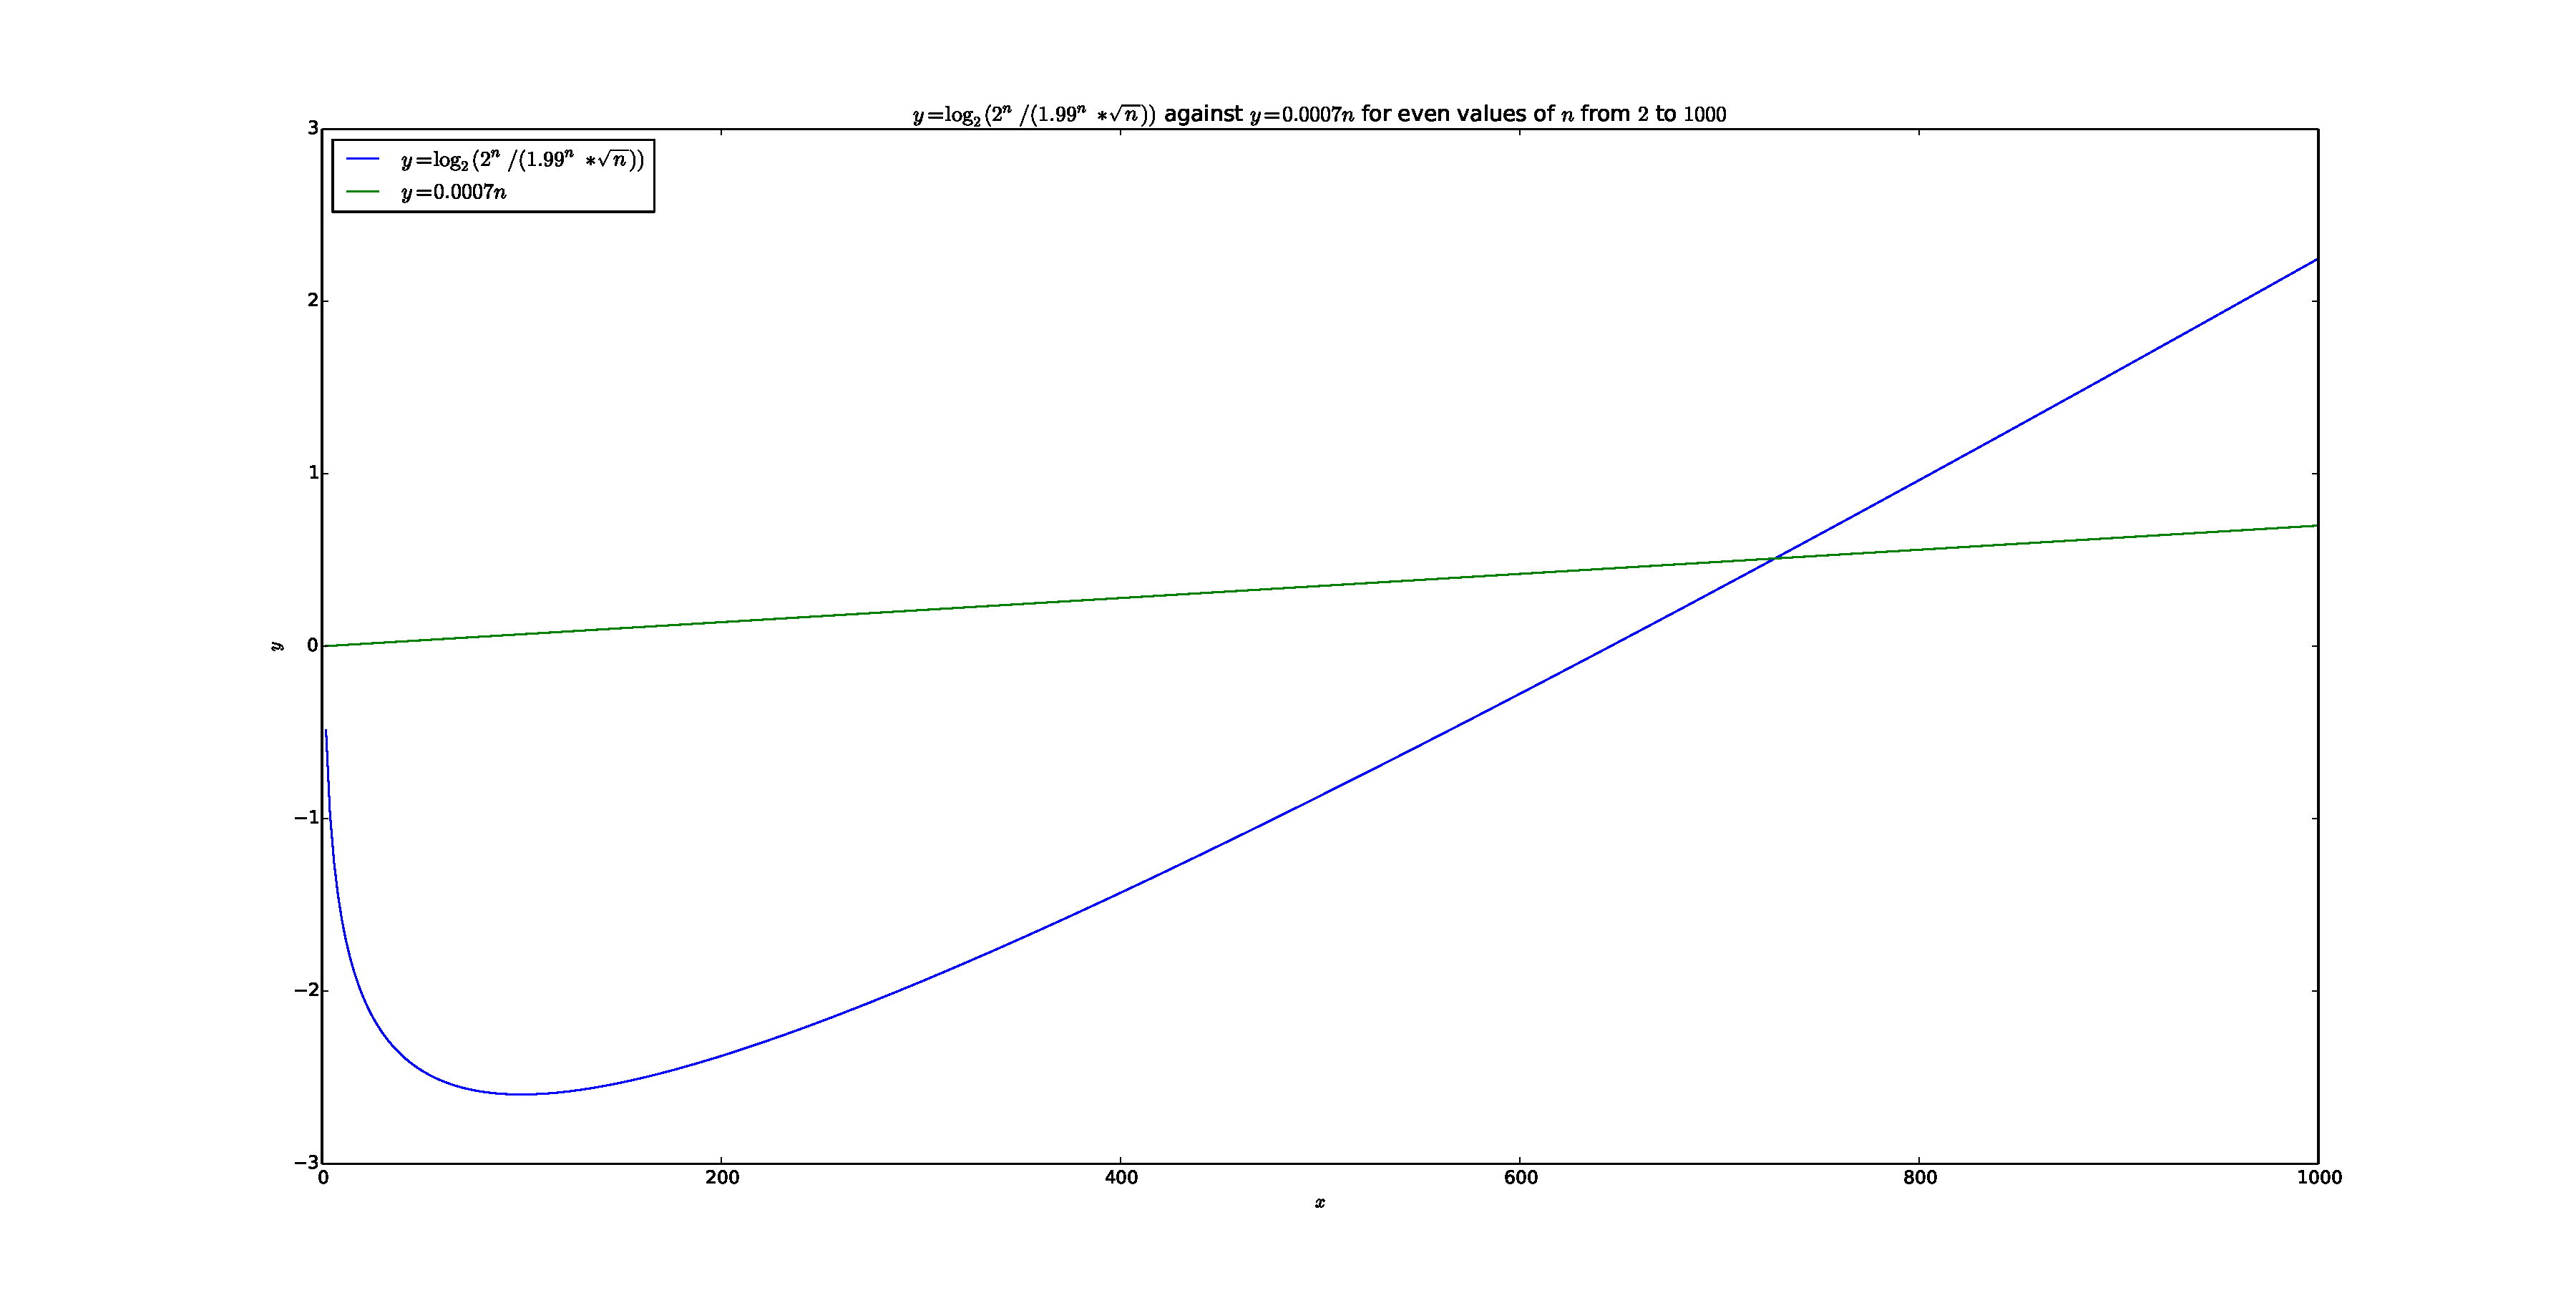
\includegraphics[width=\linewidth]{ddj_bound}
            \caption{Plot of lower bounds of Distributed Deutsch-Jozsa for $n \in \{2, 4,..., 998, 1000\}$}
            \label{fig:ddj-bound}
        \end{figure}

    \section{Lower Bound for Hidden Matching}
    \label{sec:hm-lower-bound}

    \begin{proof}[Proof of Theorem~\ref{thm:hm}]
        Take any protocol for computing the Hidden Matching Problem with mean probability of failure $\delta$ across Alice and Bob's input. If we pick a certain input for Alice $x$, we will denote the probability of error given $x$ as $\hat{e}_x$. By Markov's inequality, $Pr[\hat{e}_x \geq 2\delta] \leq \mathbb{E}[\hat{e}_x]/2\delta = \delta/2\delta = 1/2$, so at most half of Alice's inputs can fail more than $\delta/2$ of the time.

        Assuming Alice's message to Bob is written deterministically, we define the set of Alice's inputs that map to a message $\tau$ and have error less than $2\delta$ as $S_{\tau}$. Note that $\sum_{\tau}S_{\tau}$ is equal to the number of Alice's inputs with error less than $2\delta$. Using Markov's inequality above, this sum must be greater than $2^{n-1}$. Bar-Yossef, Jayram and Kerenidis then showed that for any message $\tau$, the size of the set $S_{\tau}$ is at most $2^{\Omega(n - \sqrt{n})}$. Combining these two inequalities, the number of unique messages Alice could send to Bob is at least $2^{n - 1}/2^{n - \Omega(\sqrt{n})} = 2^{\Omega(\sqrt{n}) - 1} = 2^{\Omega(\sqrt{n})}$. Assuming Alice's input is chosen uniformly at random, the length of each message must be at least $\Omega(\sqrt{n})$ classical bits. This bound is tight if public random bits are shared between Alice and Bob, as Alice can send $O(\sqrt{n})$ bits $x_i$, where $i$ is chosen from the random string. By the birthday paradox, the expected probability that a pair of indices were in Bob's matching is $1$.
    \end{proof}

    \section{Permutation Invariance}
    \label{sec:perm-invariance}

        Permutation Invariance is a problem first studied in the context of communication complexity by Montanaro \cite{Montanaro:2011:NES:2230916.2230919}, and has connections both to the Hidden Subgroup Membership problem discussed in Section~\ref{sec:subgroup-membership} and the Hidden Matching problem discussed in Section~\ref{sec:hidden-matching}.

        Let $M$ be an $n \times n$ permutation and $x$ be an $n$-bit string. We define the $n$-bit string $Mx = x_{M_i}$ for $i \in \{0,...,n-1\}$. We also define $d(a, b) = \sum_{i \in n}(a_i \oplus b_i)$ as the Hamming distance between $a$ and $b$. The problem and its quantum protocol are explained below for a parameter $\beta$:

        \begin{codebox}
            \Procname{Protocol $\proc{PERMUTATION-INVARIANCE}$}
            \zi \const{Alice's input}: $x \in \{0,1\}^n$.
            \zi \const{Bob's input}: an $n\times n$ permutation $M$.
            \zi \const{Promise}: $Mx = x$ or $d(Mx, x) \geq \beta|x|$.
            \zi \const{Bob's output}: $0$ if $Mx = x$, $1$ otherwise.
            \li Alice sends the state $|\psi_x\rangle = \frac{1}{\sqrt{x}}\sum_{i, x_i=1}|i\rangle$ to Bob.
            \li Bob adds an ancilla qubit in the state $\frac{1}{\sqrt{2}}(|0\rangle + |1\rangle)$.
            \li Bob applies the operation $M = \sum_{i \in \{0,...,n-1\}}|M_i\rangle\langle i|$ controlled on the ancilla qubit.
            \li Bob applies a Hadamard to the ancilla qubit and measures in the computational basis.
            \li If Bob measures $0$ they output $0$, otherwise they output $1$.
        \end{codebox}

        This protocol can be completed using $O(\log n)$ qubits of communication.

        The state after step 2 of the operation is $(|0\rangle|\psi_x\rangle + |1\rangle|\psi_x\rangle)/\sqrt{2}$. After applying the controlled $M$ gate, this becomes $(|0\rangle|\psi_x\rangle + |1\rangle|\psi_{Mx}\rangle)/\sqrt{2}$, where $|\psi_{Mx}\rangle = \sum_{i, x_i = 1}|M_i\rangle$. If $Mx = x$ then $|\psi_{Mx}\rangle = |\psi_x\rangle$, so the state is not changed and Bob measures $0$ with absolute certainty.

        If $Mx \neq x$ on the other hand, then the state after step 4 becomes

        $$\frac{1}{2}(|0\rangle(|\psi_x\rangle + |\psi_{Mx}\rangle) + |1\rangle(|\psi_x\rangle - |\psi_{Mx}\rangle)).$$

        The probability of measuring $0$ in this case is $\frac{1}{4}||\psi_x\rangle + |M\psi_x\rangle\|_2^2 = \frac{1}{2}(1 + \langle\psi_{Mx}|\psi_x\rangle)$\footnote{Since our amplitudes are real numbers, $\langle\psi_{Mx}|\psi_x\rangle = \langle\psi_x|\psi_{Mx}\rangle$.}. Since $d(Mx, x) \geq \beta|x|$, we can see that $\langle\psi_{Mx}|\psi_x\rangle \leq 1 - \beta$, so this protocol fails with probability $1 - \beta/2$.

        This problem can be seen as a generalisation of subgroup membership: Alice's input is a $|G|$-bit string $x$ where $x_i = 1$ iff $i \in H$ for all $i \in G$, and Bob's permutation $M_g$ maps elements $i \in G$ to $gi$. If $g \in H$, then $M_gx = x$, otherwise $d(M_gx, x) = 2|x|$. So already there is potentially a quadratic gap between quantum and classical communication for this problem, depending on whether or not such a gap exists for subgroup membership.

        The problem also relates to Hidden Matching if we only consider permutations which are completely made of disjoint pairs -- in other words, the permutation pairs bits up and swaps those pairs. Bob can build a perfect matching $M'$ by adding edges $(i, j)$ if the permutation matrix $M$ swaps $i$ with $j$. Hence this problem can be reduced to Hidden Matching, with the difference being that Bob no longer has $w$ as an input.

        How well can we perform classically? Montanaro \cite{Montanaro:2011:NES:2230916.2230919} provided a lower bound by looking at a subproblem, where Alice has a $2n$-bit string $x$ such that $|x| = n$, Bob has a $2n \times 2n$ permutation matrix $M$ and either $Mx = x$ or $d(Mx, x) \geq n/8$. Montanaro's proof breaks the problem up into two probability distributions: $\mathcal{D}_0$ when $d(Mx, x) \geq n/8$ and $\mathcal{D}_1$ when $Mx = x$. Their conclusion was that if Alice sends fewer than $\frac{n^{7/16}}{e\textrm{ln}2} - O(\log n)$ classical bits, then $\mathcal{D}_0$ and $\mathcal{D}_1$ becomes indistinguishable from the normal distribution within constant factors, and thus the distributions are indistinguishable from each other. Thus we have the following:

        \begin{theorem}
            Any randomised one-way protocol for Permutation Invariance requires $O(n^{7/16})$ classical bits of communication.
        \end{theorem}

    \section{Other Models}
    \label{sec:other-models}

        Throughout this report we have focused on one-way communication complexity. But messaging between two parts is not the only model for distributed computation, and there are a number of other communication models which have also been studied. Some of these models are briefly summarised below.

        \subsection{Zero Communication Complexity}

        Also known as 'spooky communication complexity' \cite{quant-ph/0101005}, this is the study of distributed computation problems which can be solved using only entangled qubits, without any communication whatsoever. Complexity is measured in the number of entangled pairs that have been used during computation. Much like how Holevo's theorem limits strengths of quantum communication, Alice and Bob are limited by the non-signalling properties of entanglement.

        Zero communication complexity is strongly related to non-locality \cite{RevModPhys.82.665}. There have been a number of quantum communication problems shown to be solvable in this model of computation as well, including both the Distributed Deutsch-Jozsa problem and the Hidden Matching problem. The protocols have also been used to prove lower bounds on information complexity: If there is a protocol for computing a function with information complexity $I$, there is also a zero communication protocol for computing the same function such that the function has probability greater than $2^{-O(I)}$ of not aborting, and the protocol has high probability of succeeding on condition of it not aborting \cite{Kerenidis:2012:LBI:2417500.2417819}.

        \subsection{Simultaneous Message Passing}

        In the Simultaneous Message Passing model, Alice and Bob are given inputs $x$ and $y$, respectively, and send messages one-way to a third player called the Referee without any communication between each other. The Referee must then output $f(x, y)$ for some function $f$. Another way of picturing this model is if Alice and Bob sent a single message to each other at exactly the same time, so that one party could not have received the other parties message before sending theirs, and then for both players to output the same result $f(x, y)$.

        It is already established that total functions are exponentially separated in this model: Newman and Szegedy \cite{Newman:1996:PVP:237814.238004} proved that equality of two $n$-bit strings in this model required $O(\sqrt{n})$ bits of communication. On the other hand, Buhrman et al.~\cite{PhysRevLett.87.167902} showed that the same problem in this model could be solved in $O(\log n)$ qubits of communication. It was also shown by Gavinsky et al.~\cite{Gavinsky:2007:ESO:1250790.1250866} that $\alpha$-Matching can be solved in the Simultaneous Message Passing model using $O(\log n)$ qubits of communication.

        \subsection{Non-Local Boxes}

        Non-local boxes act as a similar resource to entanglement, where Alice and Bob are each given a black box. If Alice inputs a bit $x$ into her box, and Bob inputs a bit $y$ into his box, then Alice will get bit $a$ and Bob will get bit $b$, subject to the rule that $x \wedge y = a \oplus b$. They were first proposed by Popescu and Rohrlich \cite{10.1007/BF02058098} to see what a maximally non-local experiment would look like. Since then, several properties have been proven and summarised by Buhrman et al.~\cite{RevModPhys.82.665}. Of particular note, it was shown by van Dam \cite{Dam2012} that the existence of non-local boxes would mean that all distributed computation could be performed using a single bit of communication between parties.

        \end{appendices}

\end{document}
